% ============================================================================
\section{Seizure detection on real scalp EEG (CHB-MIT)}
\label{sec:chbmit}

After the theory phase, the first practical question was: how well do temple or ear-level electrodes detect seizures on real EEG, compared with a full cap?

\subsection{Data}

The CHB-MIT Scalp EEG Database (PhysioNet; Open Data Commons Attribution v1.0; Shoeb 2009) contains long-term paediatric recordings at 256\,Hz with bipolar 10--20 montages and clinician-marked seizure onsets and offsets. Two studies were run: a patient-specific study on 3 patients (chb01, chb03, chb05: all seizure recordings plus 6 seizure-free files each; 19 seizures, 36.6\,h), and a general-model study on all subjects (chb01 and chb21 are the same child and were merged, giving 23 subjects; every seizure recording plus 3 seizure-free recordings per subject; 207 recordings, 185 seizures, 297\,h).

\subsection{Detection pipeline}

All steps are causal (usable in real time on a device):
\begin{enumerate}
\item Band-pass 0.5--45\,Hz (4th-order Butterworth); 2\,s windows every 1\,s, each scored at its end.
\item 14 features per channel: line length, log variance, Hjorth mobility and complexity, log band power in $\delta$ (0.5--4), $\theta$ (4--8), $\alpha$ (8--13), $\beta$ (13--30), $\gamma$ (30--45\,Hz), and the five relative band powers.
\item HistGradientBoosting (150 trees, learning rate 0.1, 31 leaves, class-balanced).
\item Causal 5\,s moving average of the probability, alarm on crossing a threshold, then a 60\,s refractory period.
\end{enumerate}
Event metrics: a seizure is detected if an alarm fires between 15\,s before onset and the seizure end; alarms within 60\,s after a seizure are not false alarms; sensitivity, false alarms per 24\,h (FA/day) and latency (alarm minus onset) are reported.

\subsection{Patient-specific study (3 patients, 19 seizures, 36.6 h)}

Montages: the full 18-channel bipolar cap; ``both temples'' (4 channels: T7--FT9, F7--T7, FT10--T8, F8--T8; FT9/FT10 sit just in front of the ears); right temple (FT10--T8, F8--T8); left temple (T7--FT9, F7--T7); right temple single channel (FT10--T8). Evaluation was leave-one-recording-out (each hour tested by a model that never saw it) and, for comparison, cross-patient (train on the other two patients).

\begin{table}[H]
\centering\small
\caption{CHB-MIT, 3 patients, threshold 0.5.}
\label{tab:chb3}
\begin{tabular}{@{}lcccccc@{}}
\toprule
& \multicolumn{3}{c}{Patient-specific} & \multicolumn{3}{c}{Cross-patient} \\
\cmidrule(lr){2-4}\cmidrule(lr){5-7}
Montage & Caught & FA/day & Latency & Caught & FA/day & Latency \\
\midrule
Full cap (18 ch) & 95\% (18/19) & \textbf{5.2} & 4.5 s & 37\% & 273.8 & 3.0 s \\
Both temples (4 ch) & \textbf{100\%} (19/19) & 9.8 & 6.0 s & 63\% & 306.6 & 18.0 s \\
Right temple (2 ch) & 100\% & 36.0 & 5.0 s & 84\% & 205.0 & 12.5 s \\
Left temple (2 ch) & 100\% & 32.1 & 10.0 s & 79\% & 414.0 & 17.0 s \\
Right temple (1 ch) & 100\% & 62.9 & 5.0 s & 100\% & 226.0 & 8.0 s \\
\bottomrule
\end{tabular}
\end{table}

Patient-specific temple montages caught every seizure, with more false alarms than the full cap (9.8 vs 5.2 per day for both temples); one-sided montages produced 3--6$\times$ more false alarms, the first evidence that \emph{both sides} matter. Cross-patient models on only two training patients generalised poorly (200--400 FA/day). With 36.6\,h, one false alarm counts as 0.66/day, so these figures are coarse, and any stricter thresholds chosen after seeing results are optimistic.

\begin{figure}[H]
\centering
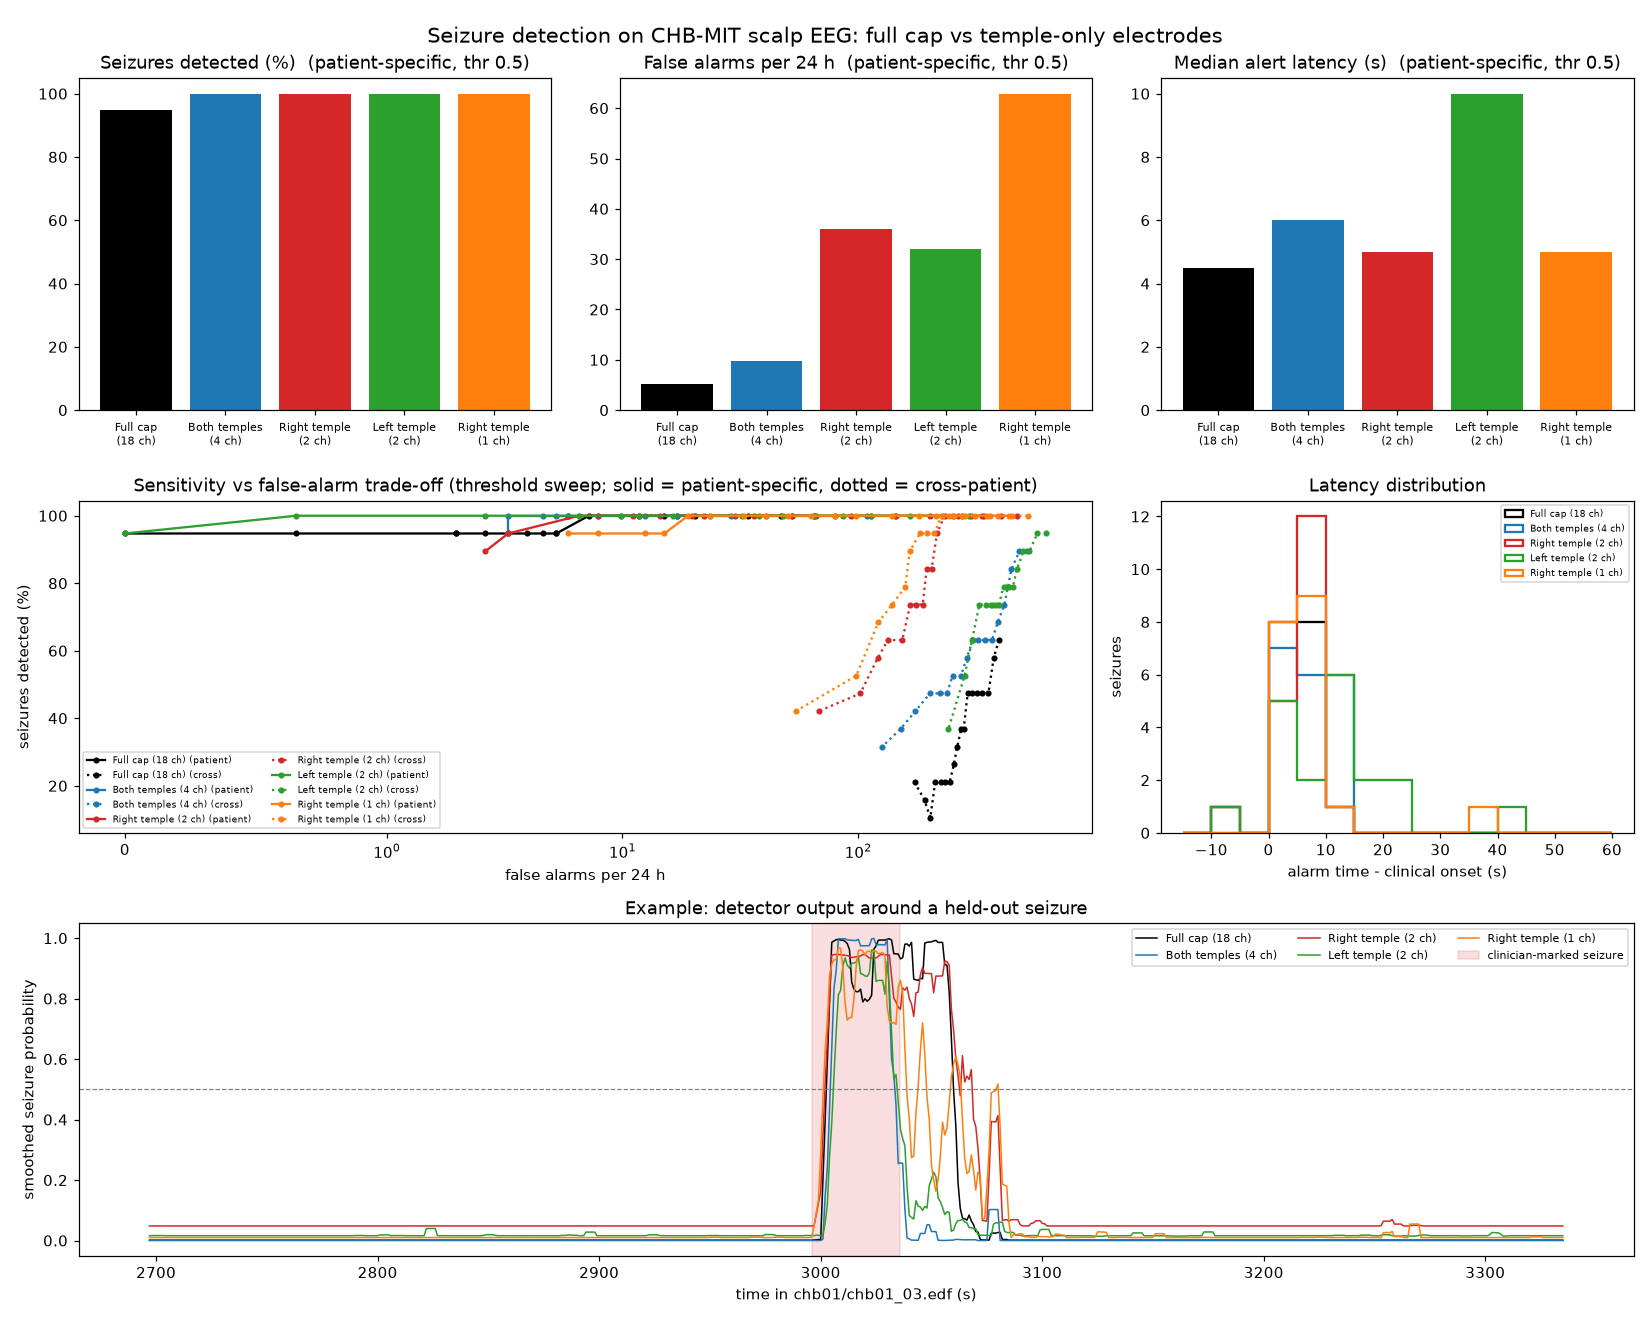
\includegraphics[width=0.8\linewidth]{epilepsy_sim/detect/results/detection.png}
\caption{CHB-MIT patient-specific detection by montage.}
\end{figure}

\subsection{General model (23 subjects, 185 seizures, 207 recordings, 297 h)}

When asked what the cross-patient table meant, and whether a \emph{general} model was possible, a new study was designed (\code{general.py}).

\paragraph{Streaming.} Each EDF was downloaded, converted to features and deleted, keeping disk use near 1\,GB. Files whose montage lacked the 18 standard channels were skipped.

\paragraph{Montages.} Temple (4 ch: F7--T7, T7--P7, F8--T8, T8--P8; FT9/FT10 are not present for every subject); \emph{ear-hook both ears} (2 ch: T7--P7, T8--P8), chosen as the closest standard channels to a ``?''-shaped ear-hook (T7/T8 just above the ear, P7/P8 above and behind it); ear-hook one ear (T8--P8); full cap (18 ch).

\paragraph{Per-person normalisation.} Each feature is z-scored against a causal exponential moving average of the same recording's previous $\approx$10 minutes (EMA over 600 one-second windows, initialised from the first minute), i.e.\ each person is compared with their own recent baseline.

\paragraph{Protocol.} Training pool: all seizure windows plus 5\% of other windows. New-user performance: leave-one-subject-out. Fine-tuning: for subjects with $\ge$3 seizure recordings and at least one seizure-free recording, the first $k$ seizure recordings (k = 1, 2) plus one seizure-free hour were added (patient weight $\times$10) and the model tested on all later recordings, compared with the general model and a patient-only model trained on the same $k$ recordings. A raw-vs-normalised ablation was run on the temple montage.

\begin{table}[H]
\centering\small
\caption{General model, new user (leave-one-subject-out), threshold 0.5.}
\label{tab:general}
\begin{tabular}{@{}lccc@{}}
\toprule
Montage & Caught & FA/day & Median latency \\
\midrule
Temple (4 ch), raw features & 62\% (114/185) & 525 & 6.5 s \\
Temple (4 ch), per-person normalised & 85\% (157/185) & 342 & 6.0 s \\
\textbf{Ear-hook both ears (2 ch)}, normalised & \textbf{88\%} (162/185) & 382 & \textbf{5.0 s} \\
Ear-hook one ear (1 ch), normalised & 83\% (154/185) & 556 & 6.0 s \\
Full cap (18 ch), normalised & 85\% (157/185) & \textbf{229} & 5.0 s \\
\bottomrule
\end{tabular}
\end{table}

\begin{table}[H]
\centering\small
\caption{Fine-tuning on the user's first $k$ seizure recordings (caught / FA per day on later recordings).}
\label{tab:generalft}
\begin{tabular}{@{}llccc@{}}
\toprule
Montage & $k$ & General only & Patient-only & General + fine-tuned \\
\midrule
Temple (4 ch) & 1 & 84\% / 351 & 53\% / 8 & 83\% / 162 \\
 & 2 & 84\% / 361 & 68\% / 16 & \textbf{86\% / 138} \\
Ear-hook both ears (2 ch) & 1 & 86\% / 385 & 54\% / 9 & 83\% / 186 \\
 & 2 & 87\% / 397 & 65\% / 18 & \textbf{86\% / 162} \\
Ear-hook one ear (1 ch) & 1 & 81\% / 547 & 44\% / 13 & 74\% / 241 \\
 & 2 & 81\% / 550 & 66\% / 79 & 80\% / 216 \\
Full cap (18 ch) & 1 & 83\% / 240 & 56\% / 3 & 84\% / 95 \\
 & 2 & 84\% / 246 & 68\% / 6 & \textbf{89\% / 88} \\
\bottomrule
\end{tabular}
\end{table}

At stricter thresholds (chosen after seeing results, hence optimistic), fine-tuned detectors reached $\approx$18--23 FA/day while catching 64\% (ear-hook both ears) to 75\% (full cap) of seizures.

\begin{figure}[H]
\centering
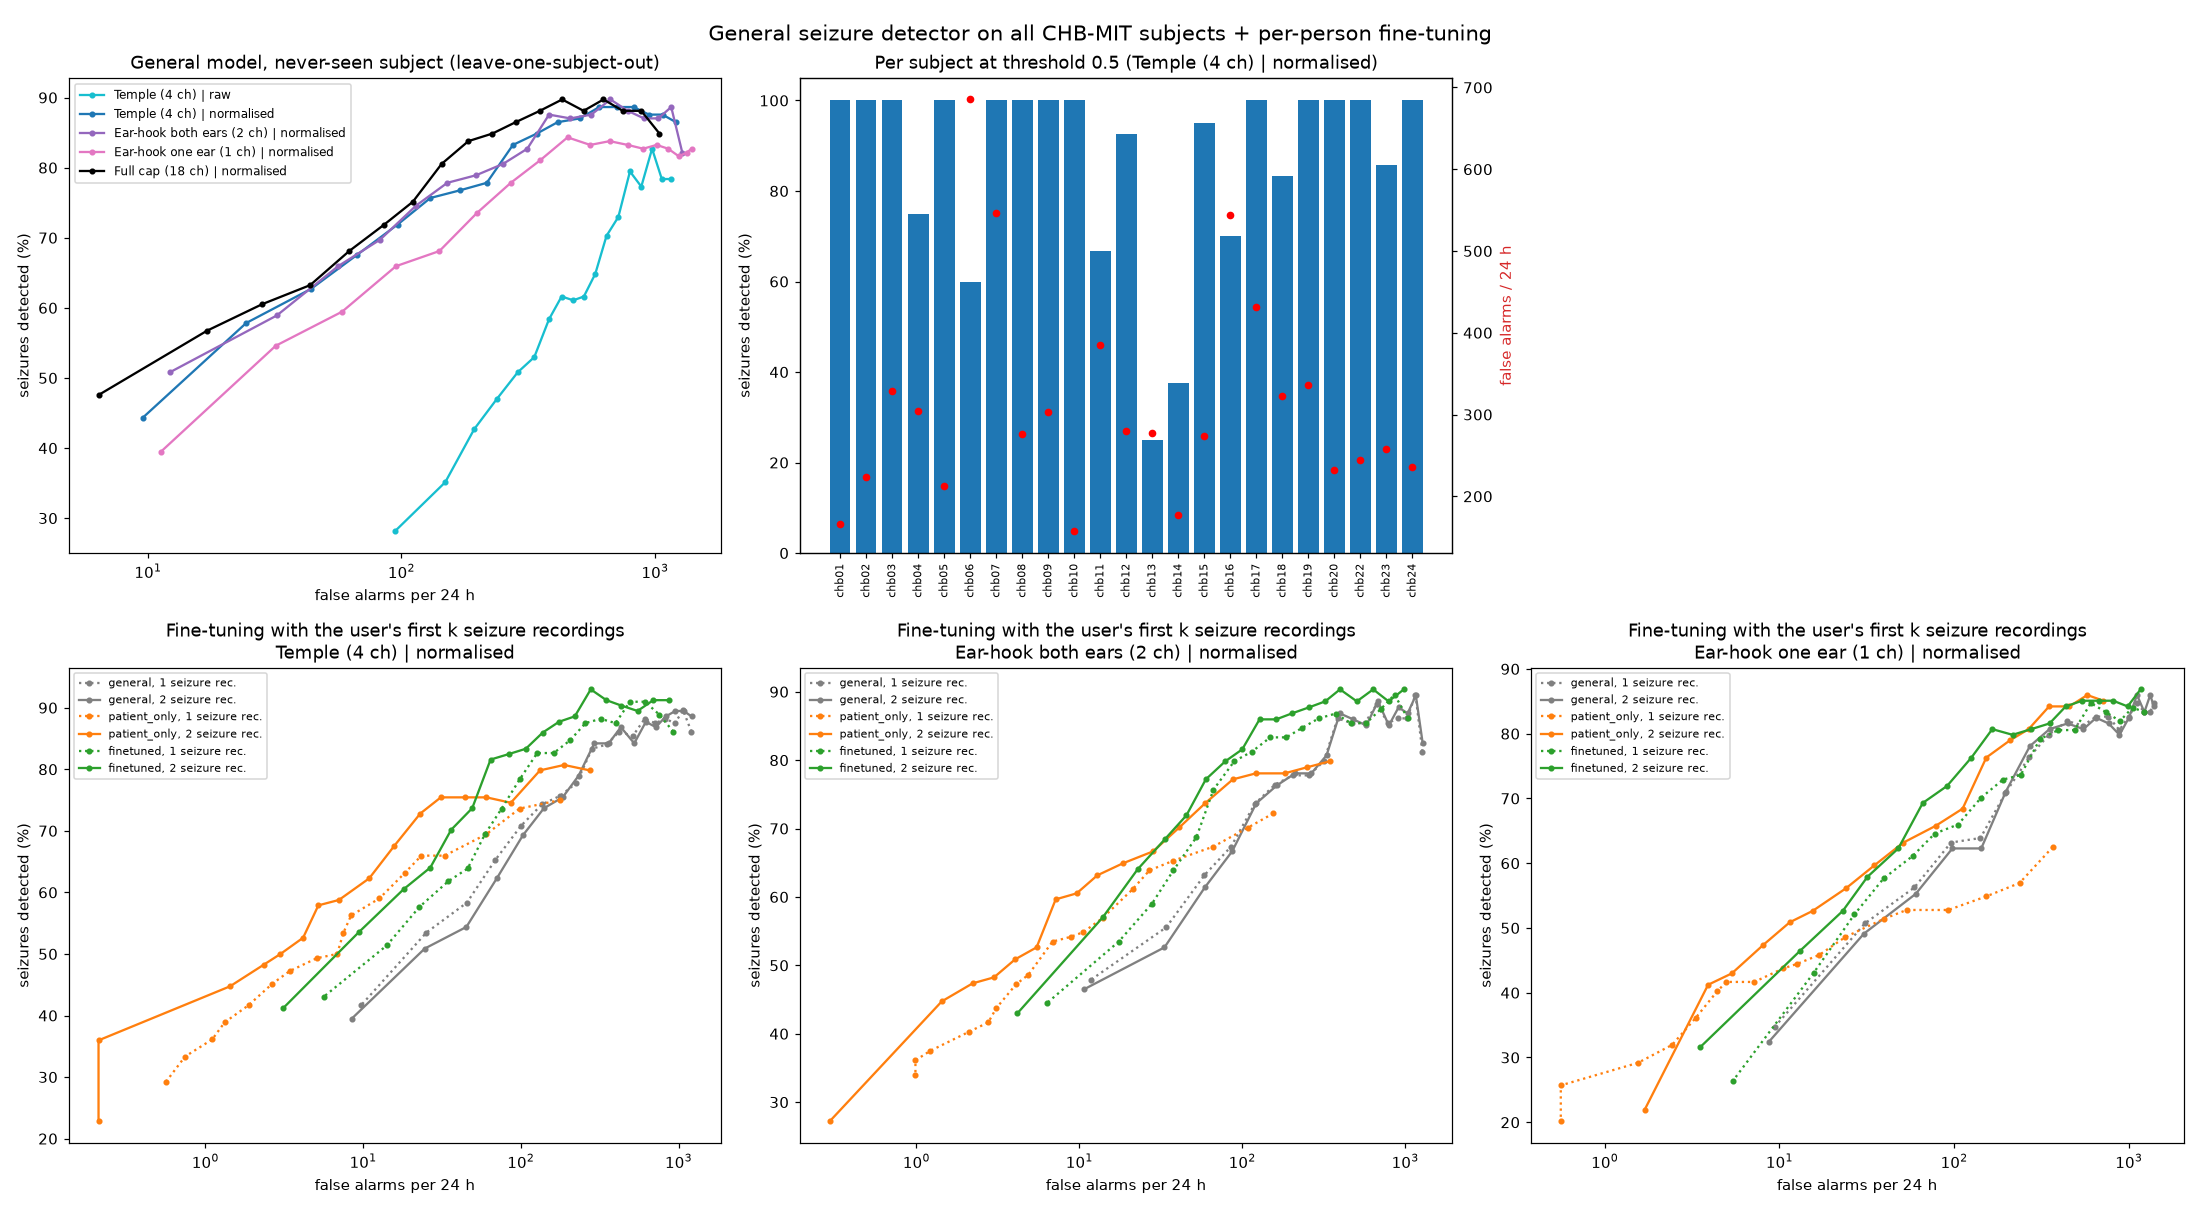
\includegraphics[width=0.95\linewidth]{epilepsy_sim/detect/results_general/general.png}
\caption{General model on all CHB-MIT subjects and personal fine-tuning.}
\end{figure}

\paragraph{Findings.}
\begin{enumerate}
\item Per-person normalisation added 43 detected seizures to the temple montage (62\%$\to$85\%) while reducing false alarms.
\item Fine-tuning on two own seizure recordings cut false alarms by 40--65\% without losing seizures.
\item The two-channel ear-hook matched the four-channel temple montage and caught as many seizures as the 18-channel cap (88\% vs 85\%); the extra channels mainly buy false-alarm rejection ($\approx$2$\times$ fewer).
\item Both ears beat one ear: about 6\% more seizures and 25--30\% fewer false alarms.
\item Patient-only models had few false alarms but missed about a third of seizures; two examples are too few to learn from alone.
\item Absolute false-alarm rates (hundreds per day for new users) were far too high: the decisive motivation for adding body signals.
\end{enumerate}

\subsection{Operational issues and fixes}

PhysioNet downloads ran at $\approx$153\,KB/s, so the AWS open-data mirror was used. File \code{chb02_16+.edf} returned HTTP 404 until its name was URL-encoded; network errors were made non-fatal and retried on the next run. Long runs inside the assistant's session were repeatedly killed by memory-pressure reaping, so heavy jobs were thereafter run by the user in their own terminal, with resumable checkpoints (results saved as soon as each configuration's general stage finished; per-configuration random seeds from a CRC32 of the name). A \code{tqdm.write(flush=...)} keyword crashed a run and was removed. A PNG locked by an image viewer triggered a timestamped fallback file. Phone notifications (ntfy) announced completion, crashes or stopped processes; a small notifier script also served as the requested ``phone call'' feature.
